\section*{Тренировочное задание}

В соответствии с \textbf{вариантом 1} необходимо осуществить планирование проекта, временные характеристики которого представлены в таблице~\ref{tbl:t_1}.

\captionsetup{justification=raggedright,singlelinecheck=off}
\begin{table}[h]
    \caption{\label{tbl:t_1}Временные характеристики проекта}
    \begin{center}
        \begin{tabular}{|c|c|}
                    \hline
              \textbf{Название работы} & \textbf{Длительность (дни)}            \\ \hline
            Работа A  & 12    \\ \hline
            Работа B & 6    \\ \hline
            Работа C  & 10    \\ \hline
            Работа D  & 7    \\ \hline
            Работа E  & 9    \\ \hline
            Работа F  & 8    \\ \hline
            Работа G  & 10    \\ \hline
            Работа H  & 10    \\ \hline
            Работа I  & 6    \\ \hline
            Работа J  & 5    \\ \hline
            \end{tabular}
    \end{center}
\end{table}

Дата начала проекта – 1-й рабочий день марта текущего года.

Провести планирование работ проекта, учитывая следующие связи между
задачами:

\begin{enumerate}
    \item предусмотреть, что D – исходная работа проекта;
    \item работы С, E и F начинаются сразу по окончании работы D;
    \item работы A и J следуют за C, а работа G – за F;
    \item работа I следует за A, а работа B – за G;
    \item работа H начинается после завершения E, но не может начаться, пока не завершены I и B.
\end{enumerate}

\newpage 
\subsection*{Результат}

Параметры рабочей среды стандартные, представлены на рисунке~\ref{fig:u1}.

\begin{figure}[h!]
	\begin{center}
		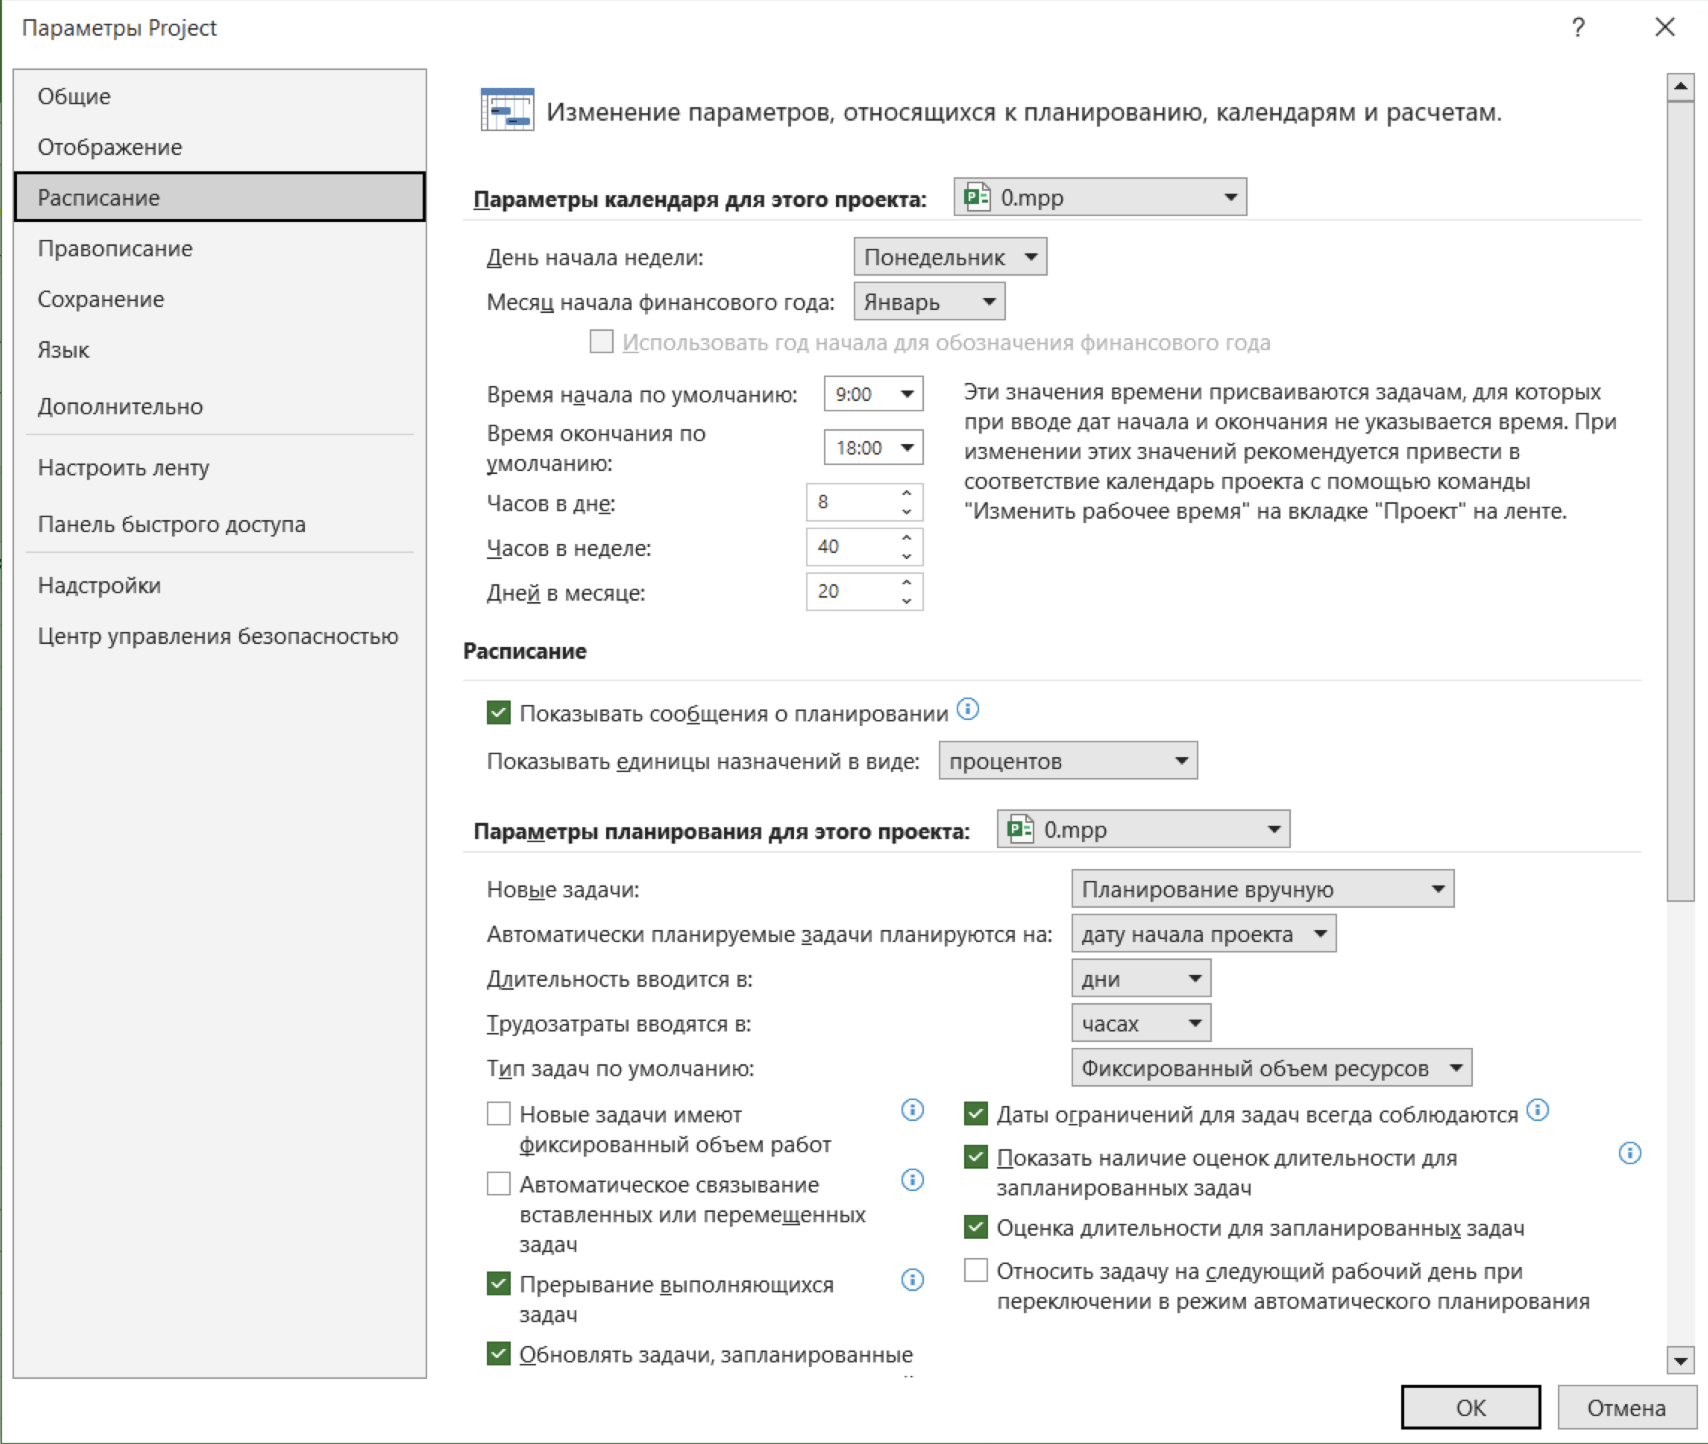
\includegraphics[scale=0.45]{inc/img/p_2.png}
	\end{center}
	\captionsetup{justification=centering}
	\caption{Параметры рабочей среды}
	\label{fig:u1}
\end{figure}

Результат планирования можно увидеть на рисунке~\ref{fig:u2}.

\begin{figure}[h!]
	\begin{center}
		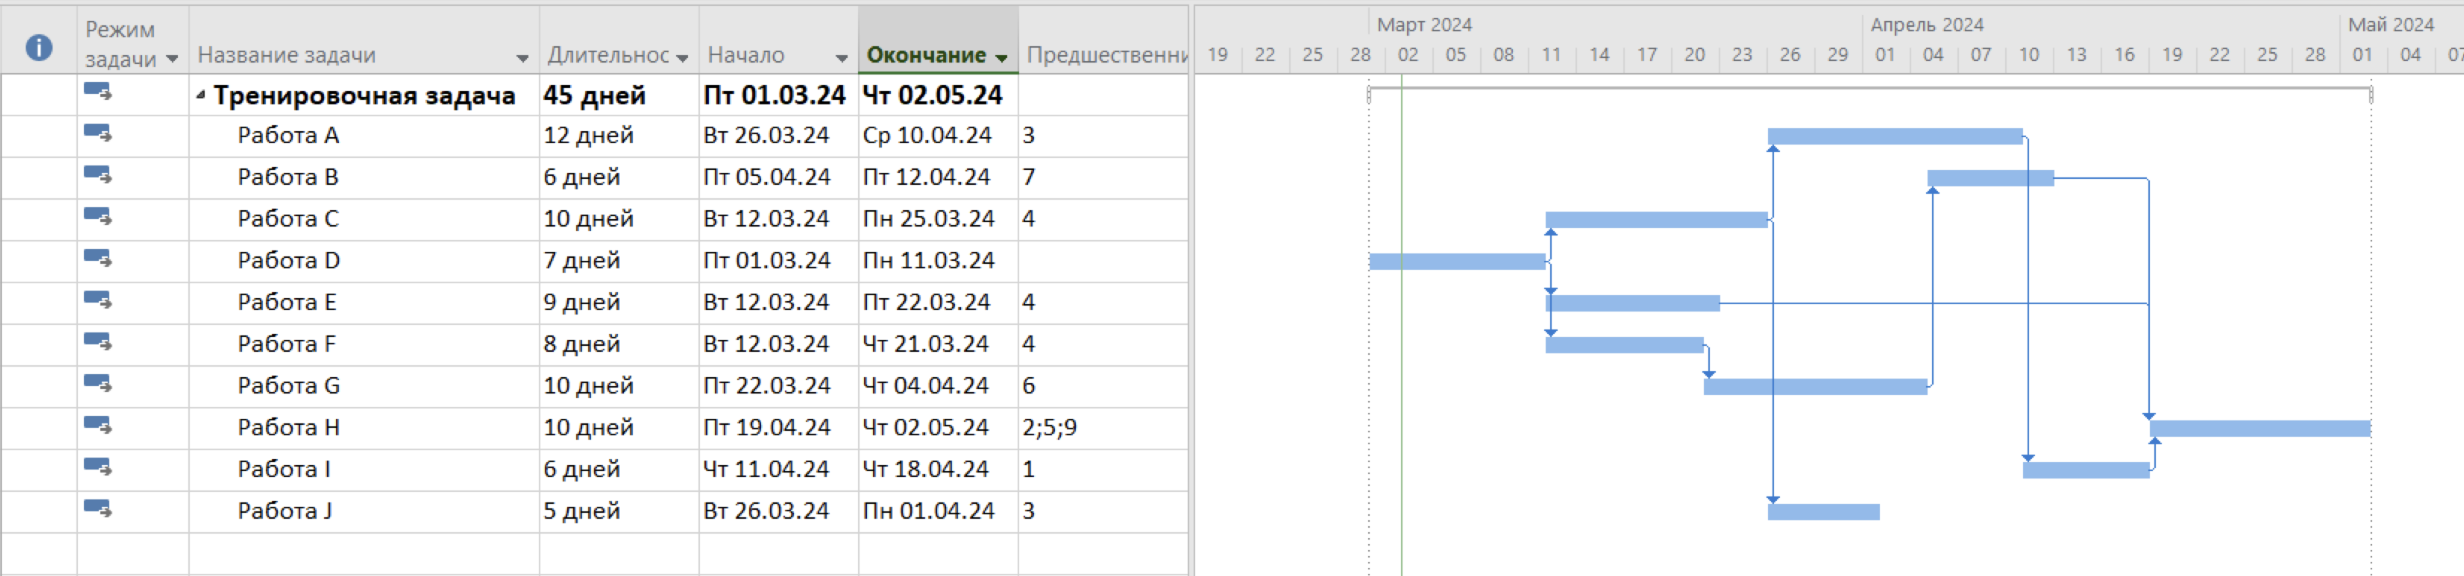
\includegraphics[scale=0.38]{inc/img/p_1.png}
	\end{center}
	\captionsetup{justification=centering}
	\caption{Результат планирования}
	\label{fig:u2}
\end{figure}

Дата начала проекта --- 01.03.24 (пятница). Дата завершения --- 02.05.24. Длительность --- 45 дней.

\begin{figure}[h!]
	\begin{center}
		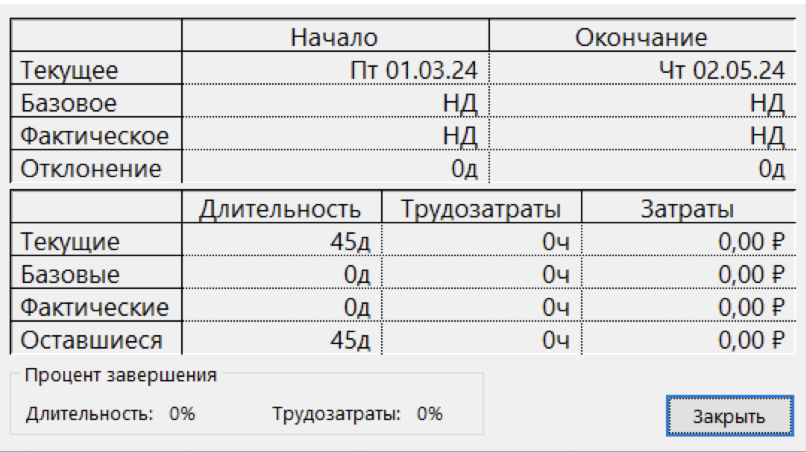
\includegraphics[scale=0.8]{inc/img/p_3.png}
	\end{center}
	\captionsetup{justification=centering}
	\caption{Статистика проекта}
	\label{fig:u3}
\end{figure}

\section*{Лабораторная работа}

\textbf{Цель работы}: освоение возможностей программы Microsoft Project для планирования
проекта по разработке программного обеспечения.



\textbf{Содержание проекта}: команда разработчиков из 16 человек занимается созданием карты города на основе собственного модуля отображения. Проект должен быть завершен в течение 6 месяцев. Бюджет проекта: 50 000 рублей.

\subsection*{Задание 1: настройка рабочей среды проекта}

На вкладке «Проект → Сведения о проекте» установлены параметры по
условию:

\begin{itemize}
    \item[(1)] дата начала проекта – первый рабочий день марта текущего года;
    \item[(6)] стандартный календарь рабочего времени.
\end{itemize}

\begin{figure}[h!]
	\begin{center}
		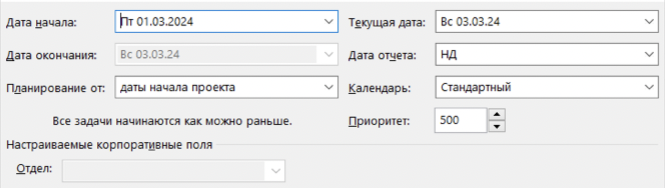
\includegraphics[scale=0.65]{inc/img/p_4.png}
	\end{center}
	\captionsetup{justification=centering}
	\caption{Настройки проекта}
	\label{fig:u3}
\end{figure}

\newpage

На вкладке «Файл → Параметры → Расписание» установлены параметры по
условию:
\begin{itemize}
    \item[(2)] длительность работы в неделях, объем работ в часах, тип работ по
умолчанию - с фиксированными трудозатратами;
    \item[(3)] количество рабочих часов в день - 8, количество рабочих часов в
неделю - 40;
    \item[(4)] начало рабочей недели в понедельник, а финансового года - в январе;
    \item[(5)] продолжительность рабочего дня с 9 до 18 часов.
\end{itemize}

\begin{figure}[h!]
	\begin{center}
		
\includegraphics[scale=0.55]{inc/img/p_6.png}
	\end{center}
	\captionsetup{justification=centering}
	\caption{Настройки проекта}
	\label{fig:u3}
\end{figure}

\begin{figure}[h!]
	\begin{center}
		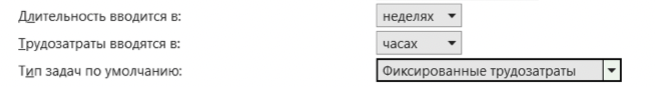
\includegraphics[scale=0.6]{inc/img/p_5.png}
	\end{center}
	\captionsetup{justification=centering}
	\caption{Настройки проекта}
	\label{fig:u3}
\end{figure}

На вкладке «Проект → Изменить рабочее время» установлены параметры по
условию:

\begin{itemize}
\item[(7)] выходные и праздничные дни на ближайшие семь-восемь
календарных месяцев от даты начала проекта.
\end{itemize}

\begin{figure}[h!]
	\begin{center}
		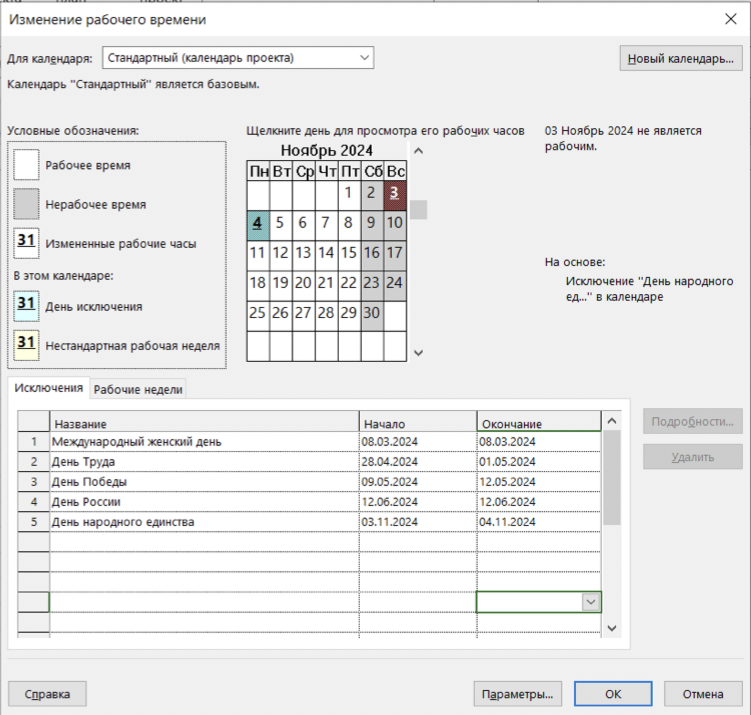
\includegraphics[scale=0.55]{inc/img/p_7.png}
	\end{center}
	\captionsetup{justification=centering}
	\caption{Настройки проекта}
	\label{fig:u3}
\end{figure}

Установлен флаг «Суммарная задача проекта»:

\begin{figure}[h!]
	\begin{center}
		
\includegraphics[scale=0.4]{inc/img/p_8.png}
	\end{center}
	\captionsetup{justification=centering}
	\caption{Настройки проекта}
	\label{fig:u3}
\end{figure}

На вкладке «Файл → Сведения → Сведения о проекте → Дополнительные
свойства → Заметки» указана информация об основных параметрах проекта
(его длительности, бюджете и количественном составе команды).

\begin{figure}[h!]
	\begin{center}
		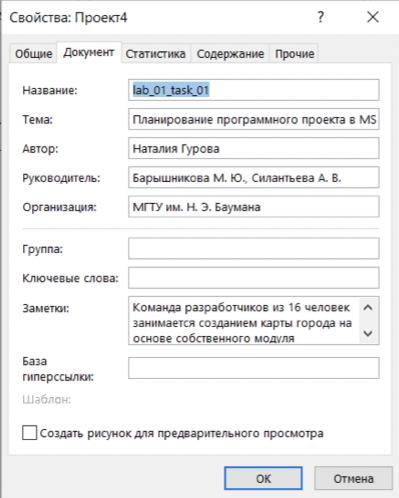
\includegraphics[scale=0.7]{inc/img/p_9.png}
	\end{center}
	\captionsetup{justification=centering}
	\caption{Настройки проекта}
	\label{fig:u3}
\end{figure}

\subsection*{Задание 2: создание списка задач}

Осуществлен ввод списка задач в соответствии с таблицей. 

\begin{figure}[h!]
	\begin{center}
		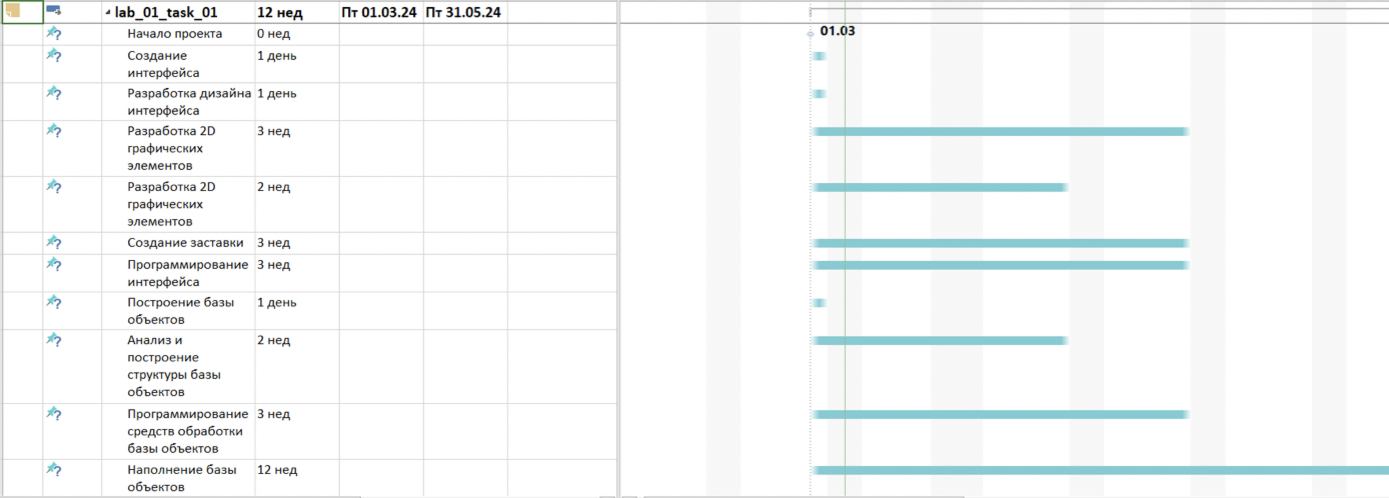
\includegraphics[scale=0.33]{inc/img/p_10.png}
	\end{center}
	\captionsetup{justification=centering}
	\caption{Список задач}
	\label{fig:u3}
\end{figure}

\newpage

\subsection*{Задание 3: структурирование списка задач}

\begin{enumerate}
    \item Проведена группировка задач 3-7 как подзадач задачи 2.
    \item Сгруппированы задачи 4-6 как подзадачи задачи 3.
    \item Проведена группировка задач 9-11 как подзадач задачи 8.
    \item Проведена группировка задач 13-16 как подзадач задачи 12.
    \item Сгруппированы задачи 20, 21 как подзадачи задачи 19.
    \item Проведена группировка задач 23-25 как подзадач задачи 22.
\end{enumerate}

\begin{figure}[h!]
	\begin{center}
		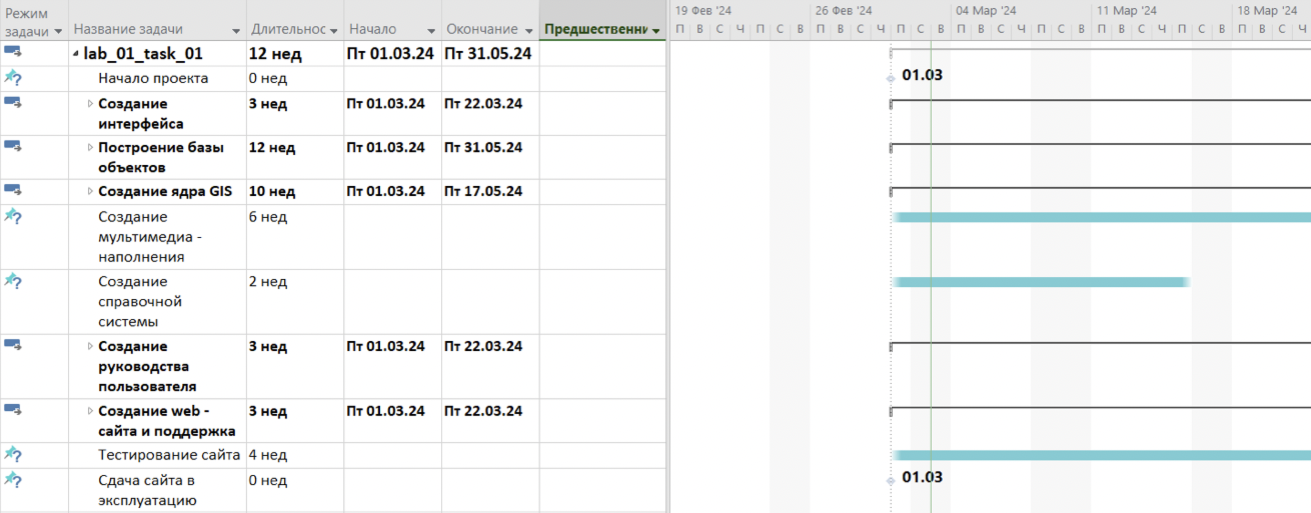
\includegraphics[scale=0.34]{inc/img/p_11.png}
	\end{center}
	\captionsetup{justification=centering}
	\caption{Структурированный список задач}
	\label{fig:u3}
\end{figure}

\subsection*{Задание 4: установление связей между задачами}

Установлены связи между работами в соответствии с таблицей.

\begin{figure}[h!]
	\begin{center}
		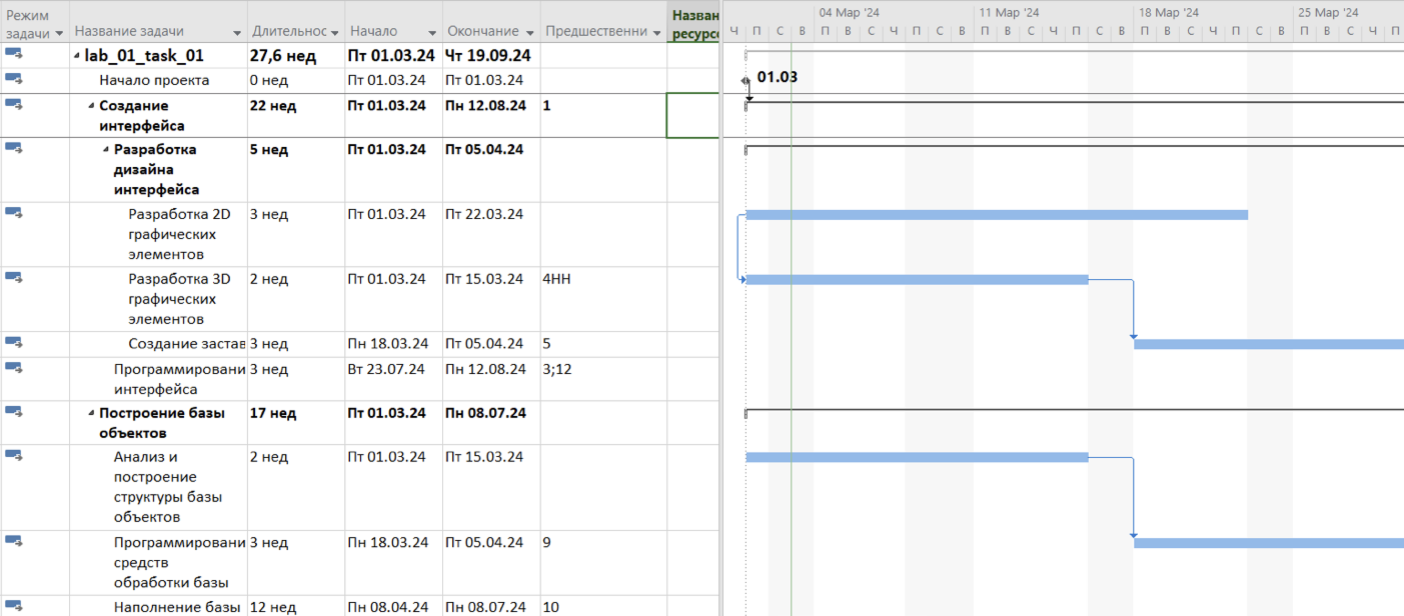
\includegraphics[scale=0.34]{inc/img/p_12.png}
	\end{center}
	\captionsetup{justification=centering}
	\caption{Связи между задачами}
	\label{fig:u3}
\end{figure}

\subsection*{Статистика по проекту}

На рисунке~\ref{fig:u10} представлена информация о дате начала и дате завершения проекта, а также длительность работы над проектом.

\begin{figure}[h!]
	\begin{center}
		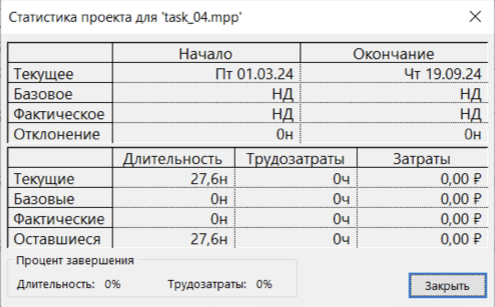
\includegraphics[scale=0.55]{inc/img/p_13.png}
	\end{center}
	\captionsetup{justification=centering}
	\caption{Дата завершения проекта}
	\label{fig:u10}
\end{figure}

\subsection*{Вывод}

Была проведена настройка рабочей среды, создание списка задач, его
структурирование и установление связей между задачами в программе MS
Project.

По описанию проекта, он должен быть завершен в течение 6 месяцев. По
расчетам при дате начала 01.03.24, проект будет завершен 18.09.24, то есть его
выполнение не укладывается в указанный срок.